\chapter{На каких языках программирования пишутся операционные системы}
\label{ch:operating-sysmets}

В главе исследуется объект Викиданных <<операционная система>> (operating system) и его свойства. В каждом из разделов представлены задачи, решённые с помощью SPARQL-запросов. В их числе: нахождение экземпляров объекта <<операционная система>>, построение списка операционных систем (ОС) по предку, по времени создания, по языку, на котором написана ОС. Также построена гистограмма, показывающая количество программ, написанных на том или ином языке программирования, и какая доля из них работает под той или иной ОС. У большого личества программного обеспечения не указан язык программирования, на котором оно разрабатывалось.


\section{Экземпляры объекта <<Операционные системы>>}
Ниже представлен SPARQL-запрос для получения списка всех операционных систем (листинг \ref{lst:all_operating_systems}).

\begin{lstlisting}[ language=SPARQL, 
caption={\href{https://w.wiki/n89}{Список всех опрационных систем}\protect\footnotemark},
label=lst:all_operating_systems
]
SELECT ?os ?osLabel
WHERE
{
	?os wdt:P31 wd:Q9135. # instance of operating system
	SERVICE wikibase:label { bd:serviceParam wikibase:language "ru, en" }
}
\end{lstlisting}
\footnotetext{Получено \num{510} операционных систем в 2017 году, и \num{1086} в 2020 году.  Ссылка на SPARQL-запрос: \href{https://w.wiki/n89}{https://w.wiki/n89}}

Наиболее полными и проработанными операционными системами на Викиданных являются: \wdqName{Linux}{388}, \wdqName{Microsoft Windows}{1406}, \wdqName{Windows 8}{5046}.

Почти пустыми и малоинформативными операционными системами оказались: \wdqName{SPIN}{16314510}, \wdqName{JavaOS}{1684163}, \wdqName{Atari TOS}{1574899}, \wdqName{Xubuntu}{72688}.

По данным ProWD у единственной в Викиданных отечественной операционной системы \wdqName{Miraculix}{4044344} заполнено 7 свойств \cite{prowd_os_link}. Лидерами по количеству заполненных свойств среди операционным системам всего мира являются \wdqName{Microsoft Windows}{1406} и \wdqName{Windows 8}{5046}, имеющие по 24 свойства.


\section{На чем основаны ОС}
В листинге \ref{lst:base_of_operating_systems} представлен SPARQL-запрос для получения списка \href{https://www.wikidata.org/wiki/Property_talk:P144}{основ (P144)} операционных систем. Данный запрос показывает соответствие между <<Операционной Системой>> и её <<предком>>, на котором она основана.


\marginnote{
	Выберите ОС, на основе которой создано больше всего других ОС:
	\begin{itemize}
		\item \href{https://w.wiki/n8U}{Debian}
		\item \href{https://w.wiki/n8V}{Android}
		\item \href{https://w.wiki/n8W}{Ubuntu}
		\item \href{https://w.wiki/n8X}{Linux kernel}
	\end{itemize}
	См. ответ~\ref{answer:what_system_created} на с.~\pageref{answer:what_system_created}.
}

\begin{lstlisting}[ language=SPARQL, 
caption={\href{https://w.wiki/n8F}{Список основ опрационных систем}\protect\footnotemark},
label=lst:base_of_operating_systems
]
SELECT ?osLabel ?baseLabel
WHERE
{
	?os wdt:P31 wd:Q9135. # instance of operating system
	?os wdt:P144 ?base. # base on 
	SERVICE wikibase:label { bd:serviceParam wikibase:language "ru, en" }
}
GROUP BY ?osLabel ?baseLabel
\end{lstlisting}
\footnotetext{Получено \num{47} результатов в 2017 году, и \num{118} в 2020 году. Ссылка на SPARQL-запрос: \href{https://w.wiki/n8F}{https://w.wiki/n8F}}


\section{Время выпуска ОС}
\marginnote{
	Какую из этих операционных систем:
	\href{https://w.wiki/n8P}{Newton OS},
	\href{https://w.wiki/n8Q}{Ubuntu Touch},
	\href{https://w.wiki/n8R}{JavaOS};
	 разработала компания \href{https://w.wiki/n8S}{Apple}?
	 
	См. ответ~\ref{answer:what_system_created} на с.~\pageref{answer:what_system_created}.
}

В листинге \ref{lst:inception_time_of_operating_systems} представлен SPARQL-запрос для получения списка операционных систем с указанием даты их создания.
\begin{lstlisting}[ language=SPARQL, 
caption={\href{https://w.wiki/n8A}{Список операционных систем с датой их создания}\protect\footnotemark},
label=lst:inception_time_of_operating_systems
]
SELECT ?osLabel ?time
WHERE
{
	?os wdt:P31 wd:Q9135. # instance of operating system
	?os wdt:P571 ?time. # inception time
	SERVICE wikibase:label { bd:serviceParam wikibase:language "ru, en" }
}
GROUP BY ?osLabel ?time
ORDER BY DESC(?time)
\end{lstlisting}
\footnotetext{Получено \num{30} результатов в 2017 году, и \num{238} в 2020 году. Ссылка на SPARQL-запрос: \href{https://w.wiki/n8A}{https://w.wiki/n8A}}

Листинг \ref{lst:inception_time_of_operating_systems} показывает в красивой графической оболочке (рисунок \ref{fig:os_creation}) таймлайн создания (на самом деле выпуска) операционных систем. А еще так-же он показывает насколько плохо заполнены Викиданные, так как в запросах выводится только 230 результатов в 2020 году. Что, в свою очередь, означает, что у других <<объектов>> поле  <<дата создания>> попросту не заполнено. Хотя информация о <<дате выпуска>> не такая уж и секретная.

\begin{figure*}[h!]
	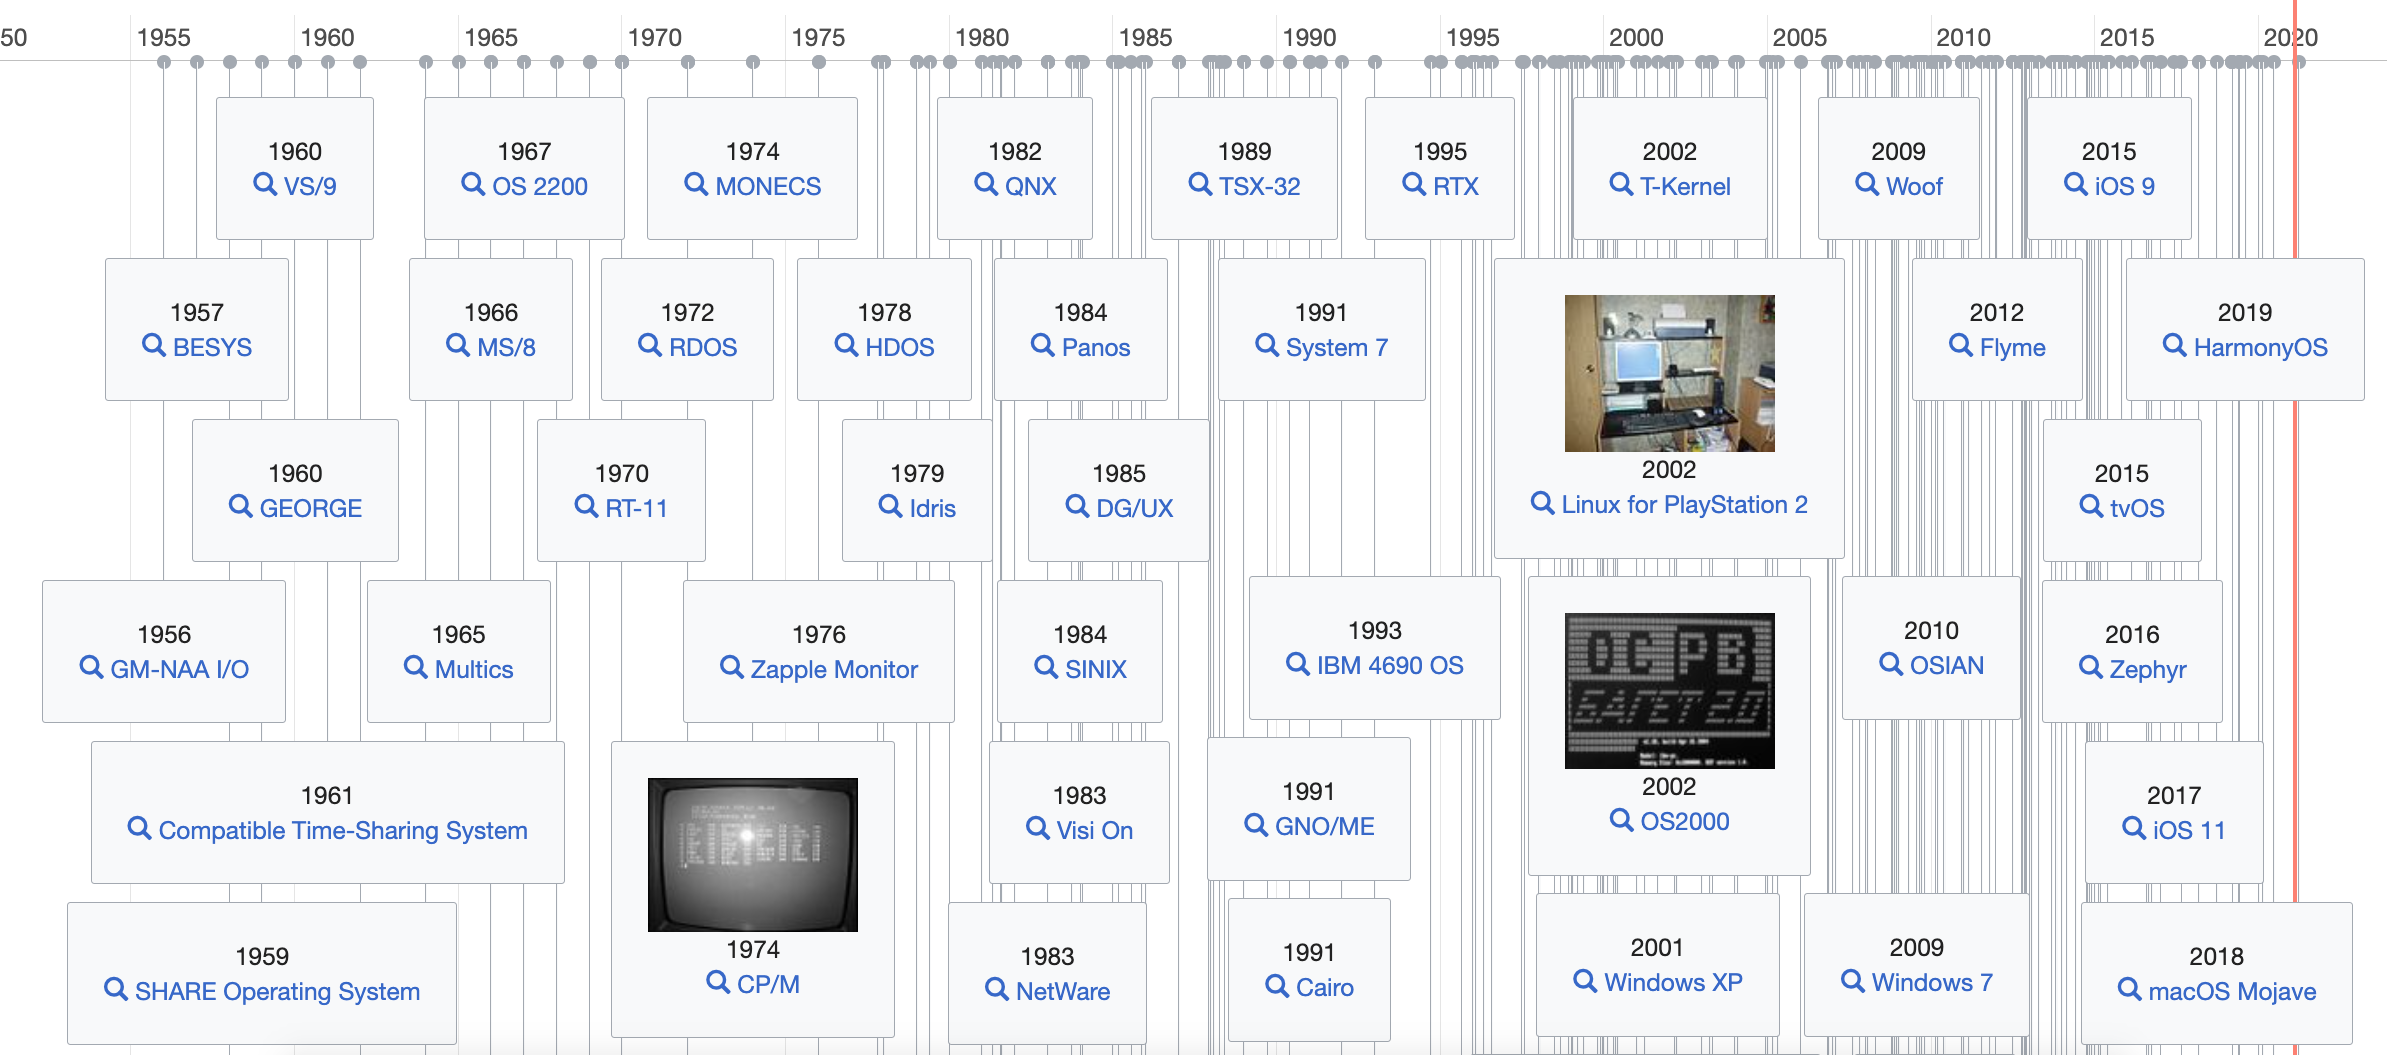
\includegraphics{./chapter/operating_system/os-creation.png}
	\caption{Часть таймлайна выпуска операционных систем на 2020 год.}
	\label{fig:os_creation}
\end{figure*}

\section{Количество ОС, написанных на языках программирования}
В листинге \ref{lst:count_os_on_languages} представлен SPARQL-запрос для получения списка языков программирования с выводом количества написанных на них ОС.

\begin{lstlisting}[ language=SPARQL, 
caption={\href{https://w.wiki/n8B}{Список языков программирования и количество написанных на них ОС}\protect\footnotemark},
label=lst:count_os_on_languages
]
SELECT ?lang (count(*) as ?count)
WHERE 
{
	?os wdt:P31 wd:Q9135. # instance of operating system
	?os wdt:P277 ?langObj. # created on programming language
	OPTIONAL {
		?langObj rdfs:label ?lang
		filter (lang(?lang) = "ru")
	}
}
GROUP BY ?lang
ORDER BY DESC(?count) ASC(?lang)
\end{lstlisting}
\footnotetext{Получено \num{24} результатов в 2017 году и \num{37} в 2020 году. Ссылка на SPARQL-запрос: \href{https://w.wiki/n8B}{https://w.wiki/n8B}}

Данный запрос показывает (только на основе заполненых викиданных, поэтому не факт что это правда) что преимущественно ОС пишут на языке Ассемблер, что несомненно является правдой, потому что это самый быстрый, но при этом удобный язык программирования. На втором и третьем месте разместились Си и C++, которые в свою очередь являются не худшим аналогом, так как несмотря на свою (относительно Ассемблера) <<медленность>>, они наиболее удобные и понятные языки программирования.


\section{Полнота данных}
По данным с сайта www.operating-system.org удалось установить что существует порядка 613 операционных систем \cite{list_operating_systems}. В то время как викиданные на 2017 год содержали информацию лишь о 510 операционных системах (не учитывая дистрибутивы Линукса, коих количество 667). И если просмотреть достаточно большое количество объектов из запросы (листинги \ref{lst:count_os_on_languages} и \ref{lst:inception_time_of_operating_systems}), то станет ясно еще и то, что много из них еще и не очень хорошо заполнены, а то и вовсе практически пусты.

В 2020 году Викиданные содержат информацию о 1086 операционных системах, что свидетельствует о значительных изменениях, однако большое количество объектов по-прежнему плохо заполнены, например по результатам запроса из листинга \ref{lst:inception_time_of_operating_systems} информация о дате выпуска заполнена всего у \num{238} языков. Из этого можно сделать вывод о неполноте Викиданных.

\section{Языки программирования, используемые для написания операционных систем}
Если взглянуть на количество операционных систем, для которых указано свойство <<язык программирования>>, то можно увидеть что из \num{1086} объектов это свойство заполнено лишь у \num{116}. Но по данным на 2020 год, представлнным на рис.~\ref{fig:count-os-written-on-languages} можно определить, что большинство операционных систем написаны на языке программирования Cи, а именно 44 ОС. 
\begin{figure*}[h!]
	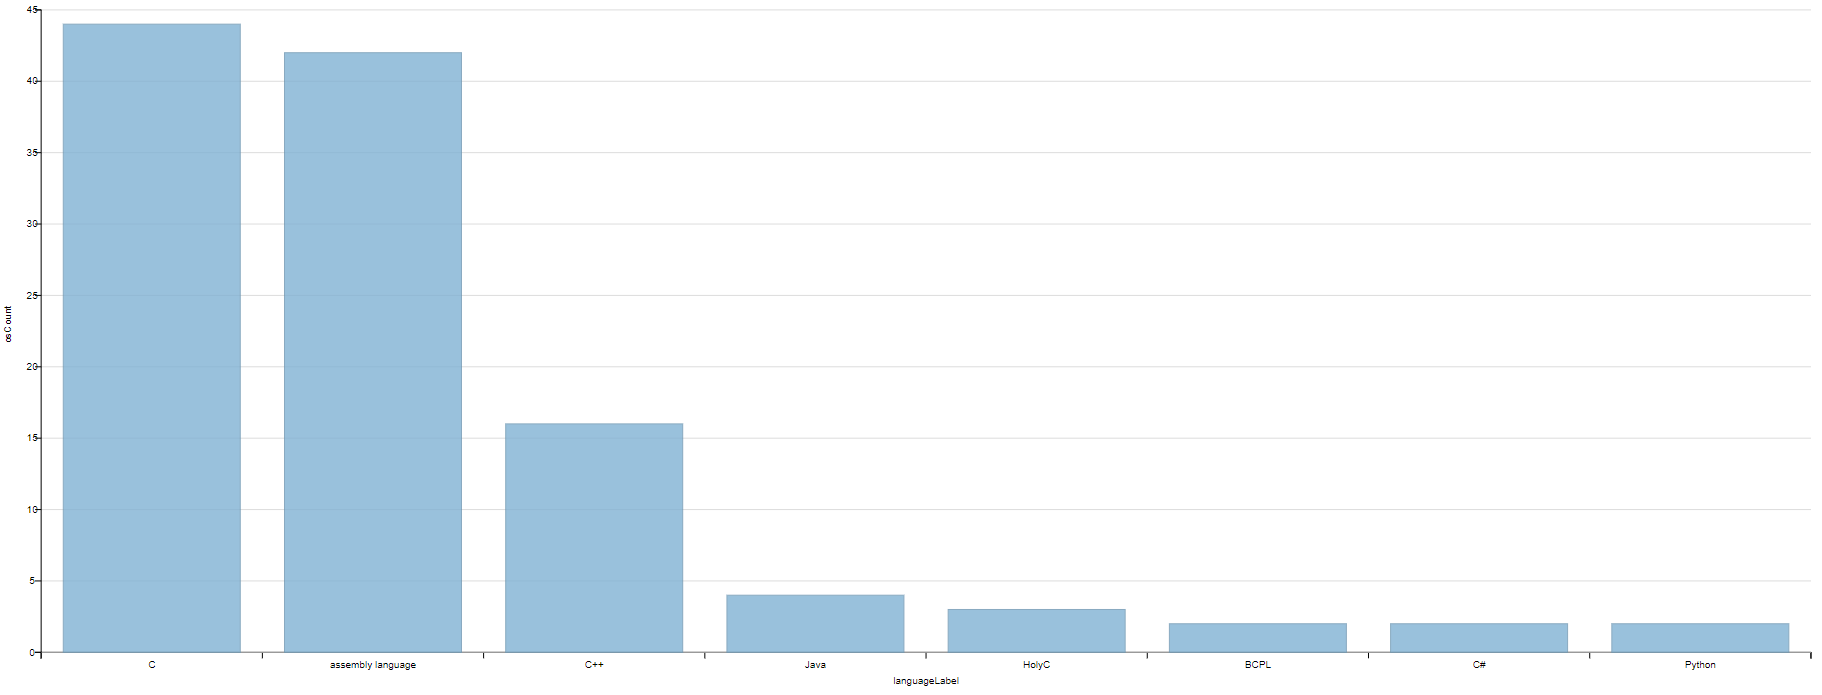
\includegraphics{./chapter/operating_system/count-os-written-on-languages.png}
	\caption{Количество операционных систем, написанных на языках программирования (данные на 2020 год.)}
	\label{fig:count-os-written-on-languages}
\end{figure*}


\section{Количество программного обеспечения под каждую ОС на скольких языках он написан}
В листинге \ref{lst:count_soft_on_os} приведен SPARQL-запрос показывающий для каждого софта под каждую ОС, на скольких языках он написан.

\begin{lstlisting}[ language=SPARQL, 
caption={\href{https://w.wiki/n8C}{Список ОС с количеством пограммного обеспеечния для него}\protect\footnotemark},
label=lst:count_soft_on_os
]
SELECT ?soft ?softLabel ?os ?osLabel (count(*) as ?count)
WHERE
{
	?soft wdt:P306 ?os. # operating system on which a software works
	?soft wdt:P277 ?lang. # programming language in which soft is developed
	SERVICE wikibase:label { bd:serviceParam wikibase:language "ru, en" }
}
GROUP BY ?soft ?softLabel ?os ?osLabel
ORDER BY DESC(?count) ASC(?lang)
\end{lstlisting}
\footnotetext{Получено \num{2259} результатов в 2017 году, и \num{6883} в 2020 году. Ссылка на SPARQL-запрос: \href{https://w.wiki/n8C}{https://w.wiki/n8C}}


\section{Сколько ПО было написано под ОС с использованием того или иного языка}
Ниже представлен SPARQL-запрос показывающий для каждого софта под каждую ОС на скольких языках он написан (листинг \ref{lst:count_soft_on_os_with_lang}).

\begin{lstlisting}[ language=SPARQL, 
caption={\href{https://w.wiki/n8D}{Список языков программирования с количеством написанного для него ПО}\protect\footnotemark},
label=lst:count_soft_on_os_with_lang
]
SELECT ?osLabel ?softLanguageLabel (count(*) as ?count)
WHERE
{
	?soft wdt:P306 ?os. # software works on os
	?soft wdt:P277 ?softLanguage. # software is written 
                                # by programming language
	?os wdt:P277 ?osLanguage. # os is written by programming language
	SERVICE wikibase:label { bd:serviceParam wikibase:language "ru, en"}
}
GROUP BY ?osLabel ?softLanguageLabel
ORDER BY DESC(?count) DESC(?osLabel)
\end{lstlisting}
\footnotetext{Получено \num{2259} результатов в 2017 году, и \num{6883} в 2020 году. Ссылка на SPARQL-запрос: \href{https://w.wiki/n8D}{https://w.wiki/n8D}}

 Данный запрос отлично показывает, что большая часть ПО, написанного под \href{https://www.wikidata.org/wiki/Q14116}{macOS}, написано на \href{https://www.wikidata.org/wiki/Q2407}{C++} (374 программы), \href{https://www.wikidata.org/wiki/Q15777}{Си} (276 программ), \href{https://www.wikidata.org/wiki/Q28865}{Python} (107 программ).
 Под \href{https://www.wikidata.org/wiki/Q94}{Android} -- \href{https://www.wikidata.org/wiki/Q2407}{C++} (107 программ) и \href{https://www.wikidata.org/wiki/Q251}{Java} (80 программ).
 Под \href{https://www.wikidata.org/wiki/Q48493}{iOS} -- \href{https://www.wikidata.org/wiki/Q2407}{C++} (63 программы).


Гистограмма на рисунке~\ref{fig:count-software-written-on-languages} позволяет увидеть для каждого языка программирования количество программ, которые были на нём написаны, а также под какими ОС работают данные программы. Из графика видно, что наибольшее число программ пишется на языках \href{https://www.wikidata.org/wiki/Q2407}{C++} (2503 программы), \href{https://www.wikidata.org/wiki/Q15777}{Си} (2566 программ), \href{https://www.wikidata.org/wiki/Q251}{Java} (799 программ), \href{https://www.wikidata.org/wiki/Q28865}{Python} (717 программ),  \href{https://www.wikidata.org/wiki/Q2005}{Javascrip} (344 программы).


\begin{figure*}[h!]
	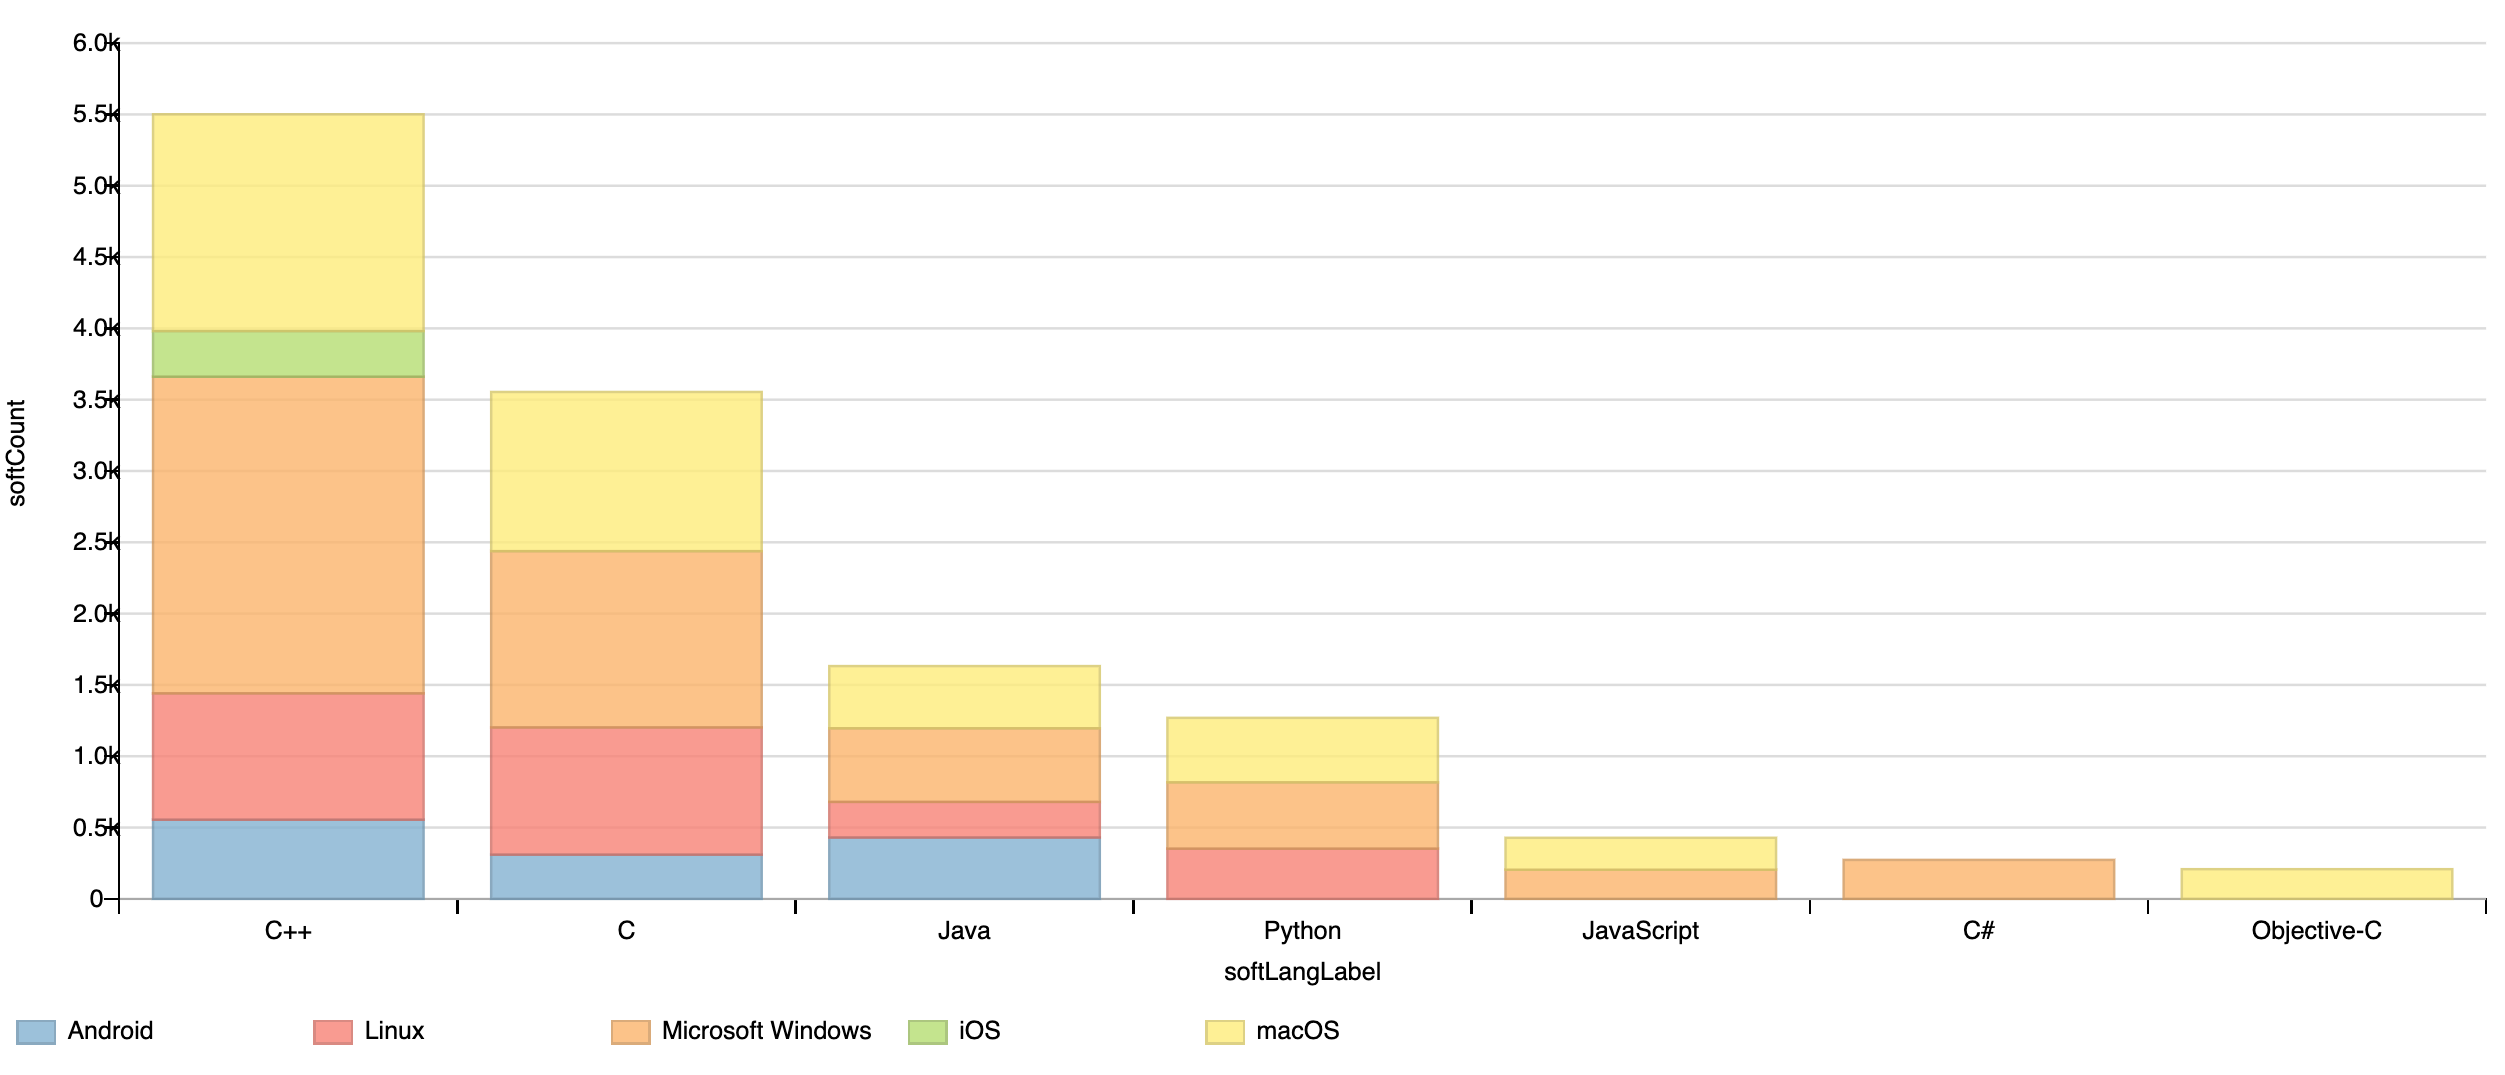
\includegraphics{./chapter/operating_system/Programming-languages-and-count-of-programms-written-on-them-and-OS-2020.png}
	\caption{Языки программирования и количества ОС, под которыми работают программы, написанные на них 2020 год.}
	\label{fig:count-software-written-on-languages}
\end{figure*}

Рассмотрим каждый из этих языков подробнее.

Большая часть программ на языке С++ пишется под Windows (472 программы) и macOs (300 программ). Несмотря на то, что язык С++ был разработан в 1972, он пока не теряет своей популярности за счет, вероятно, того, что используется для написания низкоуровневых приложений, так как по <<близости>> к аппаратному уровню уступает, разве что, ассемлеру.

Большая часть программ на языке С++ пишется под macOS (400 программ) и Windows (700 программ) и Linux (400 программ). Вероятно, С++ будет лидировать еще долгое время, так как на текущий момент он используется для решений, требующих высокой производительности, чего не позволяют высокоуровневые языки, как Java или C\#.

Большая часть программ на языке Java пишется под macOS (196 программ) и Андроид (156 программ). Вероятно, Java пользуется популярностью за счет переносимости\footnotemark \footnotetext{Переносимость -- возможность запускать код на множестве платформ без каких-либо изменений.}
кода, то есть код на Java запустится на любой машине с установленной JVM\footnotemark.
\footnotetext{Java virtual machine (JVM) — это программа, предназначенная для выполнения других программ.}

Большая часть программ на языке JavaScript пишется под macOS (100 программ) и Андроид (60 программ) и iOS (40 программ). Как правило, используется для написания клиентской части веб-приложений, что разработке сложных веб-приложений приводит к снижению нагрузки на сервер и увеличению скорости работы приложения.

Большая часть программ на языке Python пишется под macOS (212 программ) и Linux (107 программ). Используется, например, для написания веб-приложений и анализа данных.

Глядя на гистограмму, можно сделать вывод, что каждый из рассмотренных языков занял свою <<нишу>> в области разработки ПО и применяется для определенного круга задач. Также важно отметить, что большая часть ПО пишется под macOS (900 программ), Windows (1500 программ), Linux (1200 программ) или Андроид (300 программ).